\documentclass[a4paper]{article}
\usepackage[utf8]{inputenc}
\usepackage[L7x]{fontenc}
\usepackage[lithuanian]{babel}
\usepackage{lmodern}
\usepackage{amsmath}
\usepackage{graphicx}
\usepackage[top=1cm, bottom=1cm, left=1cm, right=1cm, footskip=1cm, a4paper]{geometry}
\usepackage{tasks}

\begin{document}
\begin{minipage}[b]{0.7\textwidth}
\begin{enumerate}
\item Laipsnis apibrėžiamas taip: $\underbrace{a\times a \times a \times \dots \times a}_{n} = a^n$. Kaip pasikeis šį lygybė, jei vietoje $a$ įstatysime $a^m$?
\item Paveikslėlyje pavaizduotas šiuolaikinis duomenų saugojimo metodas kompiuteriuose. Kokį dydį remiantis šiuo paveikslėliu atitinka skaičius $a^4$?

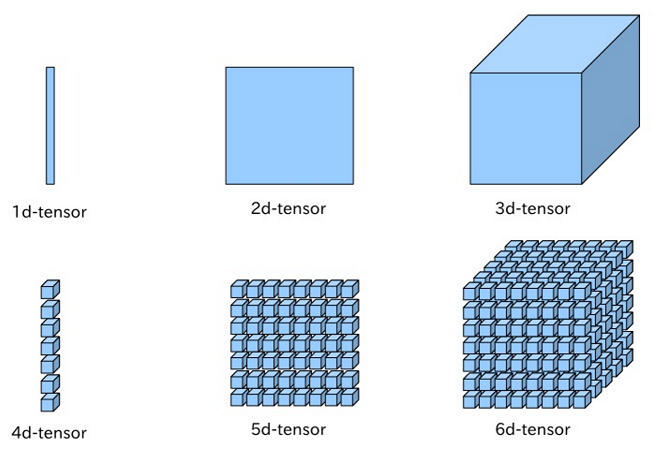
\includegraphics[width=0.4\textwidth]{tensors.png}
\item Suprastinkite reiškinius: $\underbrace{a^5+a^5+\dots+a^5}_{404}$ ir $\underbrace{a^5\times a^5\times\dots\times a^5}_{404}$
\item Kokio aritmetinio veiksmo atlikimas pavaizduotas šiame paveikslėlyje?

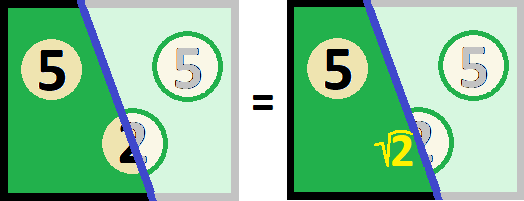
\includegraphics[width=0.4\textwidth]{rooting.png}
\item Ant to paties stalo turime dvi krūvas po tris apverstus žetonus su skaičiumi 2. Kokio veiksmo atlikimas čia pavaizduotas?
\item Skaičiaus $3^1$ laipsnio rodiklį pakeitėme į $\frac{1}{2}$, o paskui į $\frac{1}{3}$. Kokia bus gautų skaičių prasmė? Norint atsakyti užtektų nurodyti, kokios lygybės jiems galioja.
\item Ar galėtum kokiai nors taisyklei pasakyti jos dalinį atvejį?
\item Piramidė sudaryta iš pagrindo, kurio kraštinės ilgis lygus 6, o visų tos piramidės šoninių braunų ilgiai lygūs 5. Ar galėtum nustatyti tos piramidės šoninio paviršiaus plotą ir visos piramidės paviršiaus plotą?
\item Suprastinkite reiškinį $(a^2-2a+2)(a^2+2a+2)$
\item Kas yra Pitagoro trejetai? Ar galėtum keletą jų išvardinti?
\item Duota, kad dviejų kvadratų plotai sudaro trečio kvadrato plotą. Be to šie kvadratai išdėlioti taip, kad kiekvieno kvadrato kraštinė sutampa su skirtingomis to paties trikampio kraštinėmis. Kokios formos šis trikampis?
\item Prie Žemės skrisdamas dideliu greičiu priartėjo meteoras. Ar galėtum nupiešti bent keletą skirtingų netiesiaeigio judėjimo jo tolimesnio skridimo trajektorijų?
\item Išspręskite lygtis $\frac{4x^3-x^2}{x}=0$ ir $\frac{4x^3-x}{x}=0$.
\item Išskaidykite reiškinį $(2x-1)^2-1$ dauginamaisiais.
\item Apskaičiuokite: $\sqrt{54}$
\item Suprastinkite: $(x-y)(x+y)(x^2+y^2)(x^4+y^4)(x^8+y^8)$
\item \textit{\textbf{Bonus!!}} Galvosūkis karantino proga. 
\begin{enumerate}
\item Tarkime per parą užsikrėtusių skaičius vidutiniškai padidėja po $x$ vienetų, pirmą dieną buvo šimtas užsikrėtusiųjų ir praėjo dar $n$ dienų. Užrašykite reiškinį kuris parodo apytikslį užsikrėtusiųjų skaičių praėjus $n$ dienų. Po to apskaičiuokite šio reiškinio reikšmę, kai $x=10$ ir $n=30$.
\item Tarkime per parą užsikrėtusių skaičius vidutiniškai padidėja po $x$ kartų, pirmą dieną buvo šimtas užsikrėtusiųjų ir praėjo dar $n$ dienų. Užrašykite reiškinį kuris parodo apytikslį užsikrėtusiųjų skaičių praėjus $n$ dienų. Po to apskaičiuokite šio reiškinio reikšmę, kai $x=1,1$ ir $n=30$. Užuomina: skaičiavimas bus daug greitesnis, jei užrašytas reiškinys iš pradžių padauginamas iš $x-1$, o po to padalinamas.
\item Pavaizduokite abiejų augimų stulpelines diagramas
\end{enumerate} 
\end{enumerate}
\end{minipage}
\end{document}
